\documentclass{beamer}

\usetheme{simple}

\usepackage{lmodern}
\usepackage{tabularx}
\usepackage{amssymb}% http://ctan.org/pkg/amssymb
\usepackage{pifont}
\usepackage{siunitx}
\usepackage{minted}

% short cut for tick and cross commands
\newcommand{\yes}{\checkmark}
\newcommand{\no}{\hspace{1pt}\ding{55}}

\usepackage[scale=2]{ccicons}

%\setwatermark{\includegraphics[height=1.3cm]{img/watermark.jpg}}

\newcommand\pro{\item[\textbf{+}]}
\newcommand\con{\item[\textbf{--}]}

\title{Music synthesis with FPGAs \\and open-source tools}
\subtitle{}
\author{\texttt{github.com/schnommus/eurorack-pmod}}
\institute{Sebastian Holzapfel}
\date{}
\titlegraphic{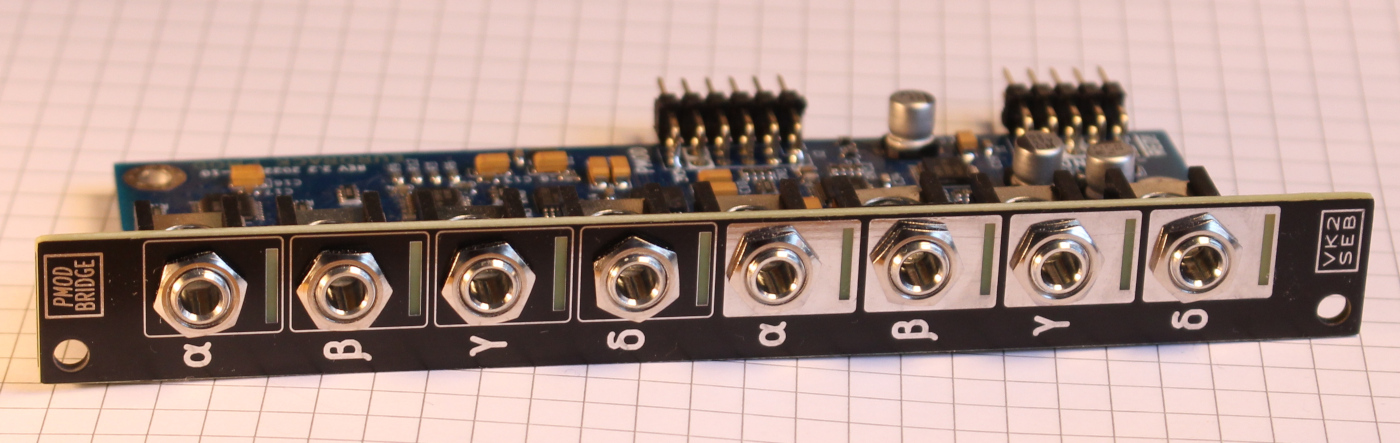
\includegraphics[height=3cm]{img/eurorack-pmod.jpg}}

\begin{document}

\maketitle

\setwatermark{}

% OUTLINE

% why eurorack?
% why eurorack-pmod?
% evolution, how it works
% (no hardware!) sim vcv & sim testbenches
% (interest?) revision 3 and manufacturing
% stay creative

% What is Eurorack?
% Simple Eurorack system (emph. DC/CV + Audio same jacks, requirements)
% Existing FPGA-based modules (v short)
% & existing development platforms (v short)

% What is EURORACK-PMOD
% Connect to any FPGA development board like such
% Lets you write simple Verilog and explore sound
% Examples in the repository (etc...)
% Specific example

% How does this work?

% INTERESTING THINGS
% HARDWARE
% - AK4619
% - Hardware evolution
% - DC coupling & calibration
%   - Misused. Price point. Fortunately outputs are DC coupled (register allows misuse)!
% - Latency
% - Light bleed mechanism
% - Revision 3
% GATEWARE
% - Simple example cores / demo
% SIMULATION
% - VCVRack demo
% - Test benches

% CUSTOM PICS/VIDS NEEDED
% - My eurorack system
% - ICEbreaker and connected to ICEbreaker
% - Latency on scope
% - Prototypes r1 2 and 3 (next to each other?)
% - VCVrack screen capture
% - 2x video demos

\begin{frame}{Outline}

    % BRIEF: who am I? / side project

    \begin{itemize}
        \item What is Eurorack?
        \item Why \texttt{eurorack-pmod}?
        \item Hardware details
        \item Writing \& simulating gateware
        \item Interest, manufacturing \& rev. 3
    \end{itemize}

\end{frame}

\begin{frame}{What is eurorack?}

    \begin{itemize}
        \item Modular system for constructing synthesizers.
        \item $>15,000$ modules, $>1,000$ different manufacturers.
    \end{itemize}

    % INSERT PICTURE (my system)

    % Routed manually by mono 3.5mm TS phono jacks

\end{frame}

\begin{frame}{A typical module}

    \begin{itemize}
        \item Modules have \textbf{input} and \textbf{output} jacks.
        \item Maximum $\pm$10V signals on \textbf{$3.5$mm mono jacks}
    \end{itemize}

    % INSERT PICTURE (module close-up with connector)

\end{frame}

\begin{frame}{Signals in the Eurorack world}

    \begin{block}{Control Voltages}
        \begin{itemize}
            \item Generally lower frequency (roughly $<1$kHz)
            \item DC absolute accuracy is important (1V/oct)
            \item \textbf{example:} drum trigger, oscillator pitch
        \end{itemize}
    \end{block}

    % INSERT PICTURE (scope capture: CV)

\end{frame}

\begin{frame}{Signals in the Eurorack world}

    \begin{block}{Audio Signals}
        \begin{itemize}
            \item Generally higher frequency
            \item Absolute accuracy not so important
            \item \textbf{example:} echo or distortion effect.
        \end{itemize}
    \end{block}

    % INSERT PICTURE (scope capture: audio)

\end{frame}

% RELATED EXISTING MODULES (do I need this?)

\begin{frame}{What is \texttt{eurorack-pmod}?}

    \begin{center}
        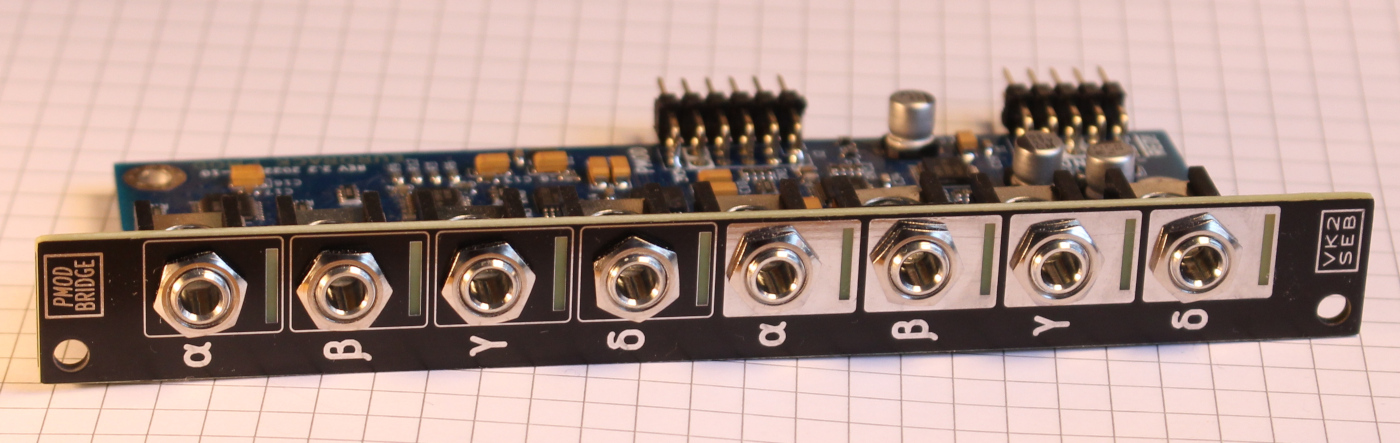
\includegraphics[height=3cm]{img/eurorack-pmod.jpg}
    \end{center}

    % The hard work is already done.
    \begin{itemize}
        \item Easy way to get started with FPGAs \& audio synthesis.
        \item PMOD connector compatible with many FPGA dev boards.
    \end{itemize}

    \begin{block}{Why?}
        \begin{itemize}
            % SAY \item Hardware, CODEC driver, calibration etc. already done.
            \item Start prototyping interesting logic straight away.
            \item Easily do things that are hard on MCU-based platforms.
                \begin{itemize}
                    \item e.g. super fast latency, tonnes of VCOs, gate-level sim of retro synth
                \end{itemize}
            \item Even for simple things, fun playground to learn FPGAs!
        \end{itemize}
    \end{block}

\end{frame}

\begin{frame}{Connected to an FPGA}

% INSERT PICTURE (Connected to ICEbreaker)
% INSERT PICTURE (Connected to ICEbreaker, in system)

\end{frame}

\begin{frame}{Gateware examples in \texttt{eurorack-pmod} repository}

    \begin{itemize}
        \item \texttt{vca.sv}: voltage controlled amplifier
        \item \texttt{vco.sv}: voltage controlled (wavetable) oscillator
        \item \texttt{sampler.sv}: simple .wav file sampler
        \item \texttt{filter.sv}: high-pass \& low-pass filter
        \item \texttt{clkdiv.sv}: clock divider
        \item \texttt{seqswitch.sv}: sequential routing switch
        \item \texttt{bitcrush.sv}: sample bit depth reducer
    \end{itemize}

\end{frame}

\begin{frame}[fragile]

    \textbf{Voltage-Controlled Amplifier}

    \begin{minted}[highlightlines={10},highlightcolor=yellow]{verilog}
module vca #(
    parameter W = 16
)(
    input signed [W-1:0] sample_in0,
    ...
    output signed [W-1:0] sample_out0,
    ...
);

assign sample_out0 = (sample_in0 * sample_in1) >>> W;

endmodule
    \end{minted}

\end{frame}

\begin{frame}{The hardware}

    % INSERT PICTURE (hardware: top down, maybe labeled)

    \begin{center}
        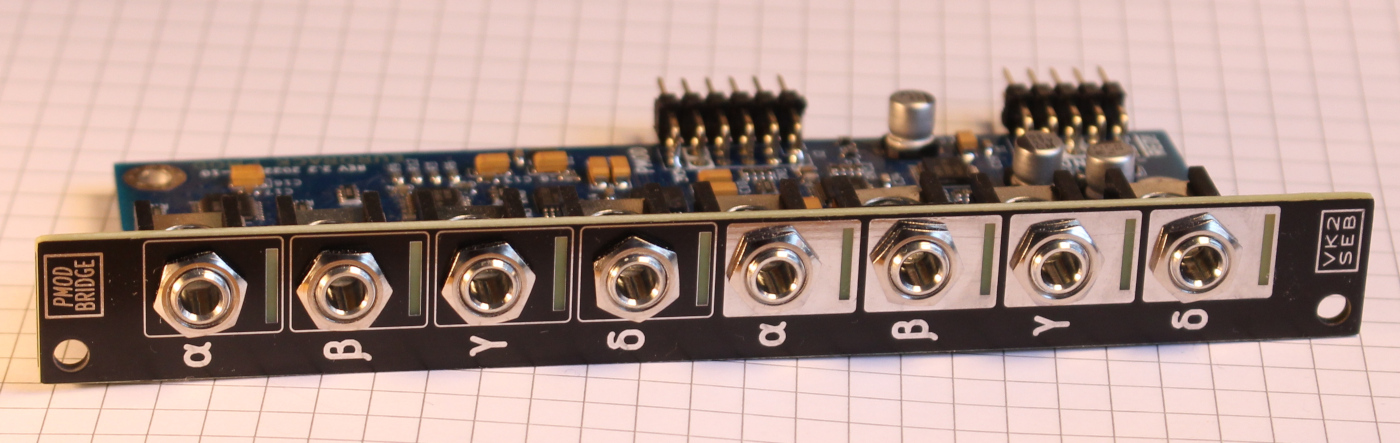
\includegraphics[height=3cm]{img/eurorack-pmod.jpg}
    \end{center}

    \begin{itemize}
        \item 4HP eurorack-compatible module with PMOD interface.
        \item 8 (4 in + 4 out) DC-coupled channels with LED indicators.
        \item 192KHz / 32bit sampling on all channels.
    \end{itemize}

\end{frame}


\begin{frame}{Hardware design}

    % INSERT 3 generations

    \begin{itemize}
        \item KiCAD files available on GitHub.
        \item Rev. 2.2 works without any bodges.
    \end{itemize}

\end{frame}

\begin{frame}{Deeper - Audio CODEC}

    % INSERT AK4619VN datasheet capture
    % OR INSERT schematic capture

    \begin{block}{AK4619VN audio codec IC}
        \begin{itemize}
            \item All 8 channels on a single I2S-like interface (fits in 1x PMOD)
            \item Much cheaper than instrumentation-quality ADCs/DACs (\$3/unit)
            \item \textbf{Can be misused in a DC-coupled mode, if calibration used}
        \end{itemize}
    \end{block}

\end{frame}

\begin{frame}{DC coupling and calibration}

    % INSERT compare input topology

    \begin{itemize}
        \item Ignore recommended input/output topology from datasheet
        \item Disable all digital high-pass filters in CODEC registers
        \item Calibrate DC extents at $\pm$ 5V, linear regression
        \item Calibrate all samples online in FPGA gateware
        % script is provided to do this (but ideally would do during mfg.)
    \end{itemize}

\end{frame}

\begin{frame}{Gateware architecture}

    \begin{center}
        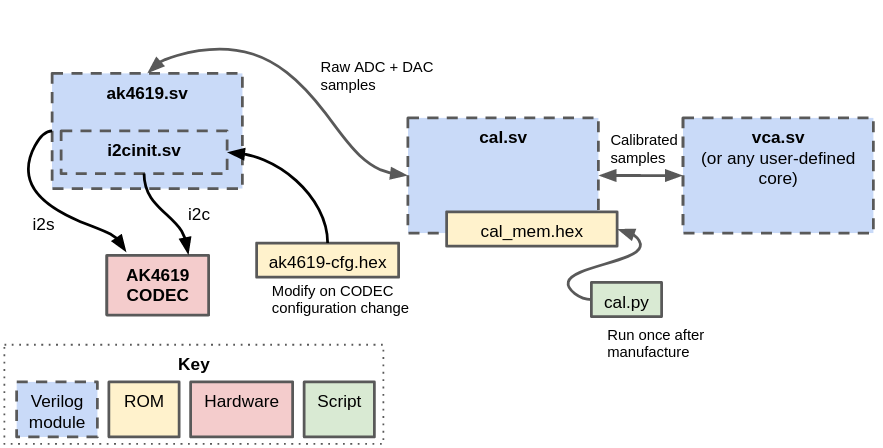
\includegraphics[height=6cm]{img/gateware-arch.png}
    \end{center}

\end{frame}

\begin{frame}{Input to output latency}

    % INSERT picture of input to output latency

\end{frame}

\begin{frame}{Simulation - VCVRack}

    \begin{center}
        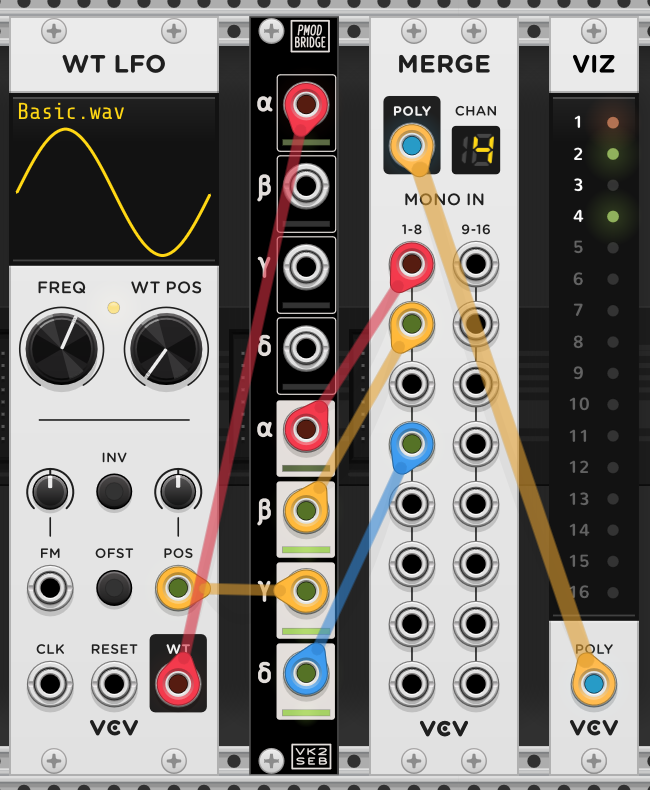
\includegraphics[height=5cm]{img/vcvrack.png}
    \end{center}

    \begin{itemize}
        \item No hardware?
        \item VCVRack plugin to \textbf{simulate verilog on a \texttt{eurorack-pmod} module}.
        \item \texttt{github.com/schnommus/verilog-vcvrack}
    \end{itemize}

\end{frame}

\begin{frame}{Manufacturing}

    \begin{block}{Revision 3 hardware}
        \begin{itemize}
            \item Jack insertion detection
            \item Calibration memory on board
            \item Leds controllable by FPGA directly
            \item Cheaper to manufacture \& lower profile
        \end{itemize}
    \end{block}

\end{frame}

\begin{frame}{Light bleed through PCB}

    % INSERT picture of LED indicators from a couple angles

\end{frame}

\begin{frame}{Thank you for listening!}

    \begin{itemize}
        \item contact: \texttt{me@sebholzapfel.com}
        \item \texttt{github.com/schnommus/eurorack-pmod}
        \item \texttt{github.com/schnommus/verilog-vcvrack}
    \end{itemize}

    \begin{block}{Help needed!}
        \begin{itemize}
            \item Is a prototype run worthwhile?
            \begin{itemize}
                \item star the GitHub repository :)
                \item register interest in `Manufacturing' section of \texttt{README.md}
            \end{itemize}
        \end{itemize}
    \end{block}

\end{frame}

\end{document}
